\section{Referencia del Archivo /media/docs/progra/c++/compiladores1/proy2/godzilla/src/colaerr.h}
\label{colaerr_8h}\index{/media/docs/progra/c++/compiladores1/proy2/godzilla/src/colaerr.h@{/media/docs/progra/c++/compiladores1/proy2/godzilla/src/colaerr.h}}
Definiciones de la cola almacenadora de errores . 

{\tt \#include $<$stdio.h$>$}\par
{\tt \#include $<$stdlib.h$>$}\par
{\tt \#include $<$string.h$>$}\par


Dependencia gr\'{a}fica adjunta para colaerr.h:\begin{figure}[H]
\begin{center}
\leavevmode
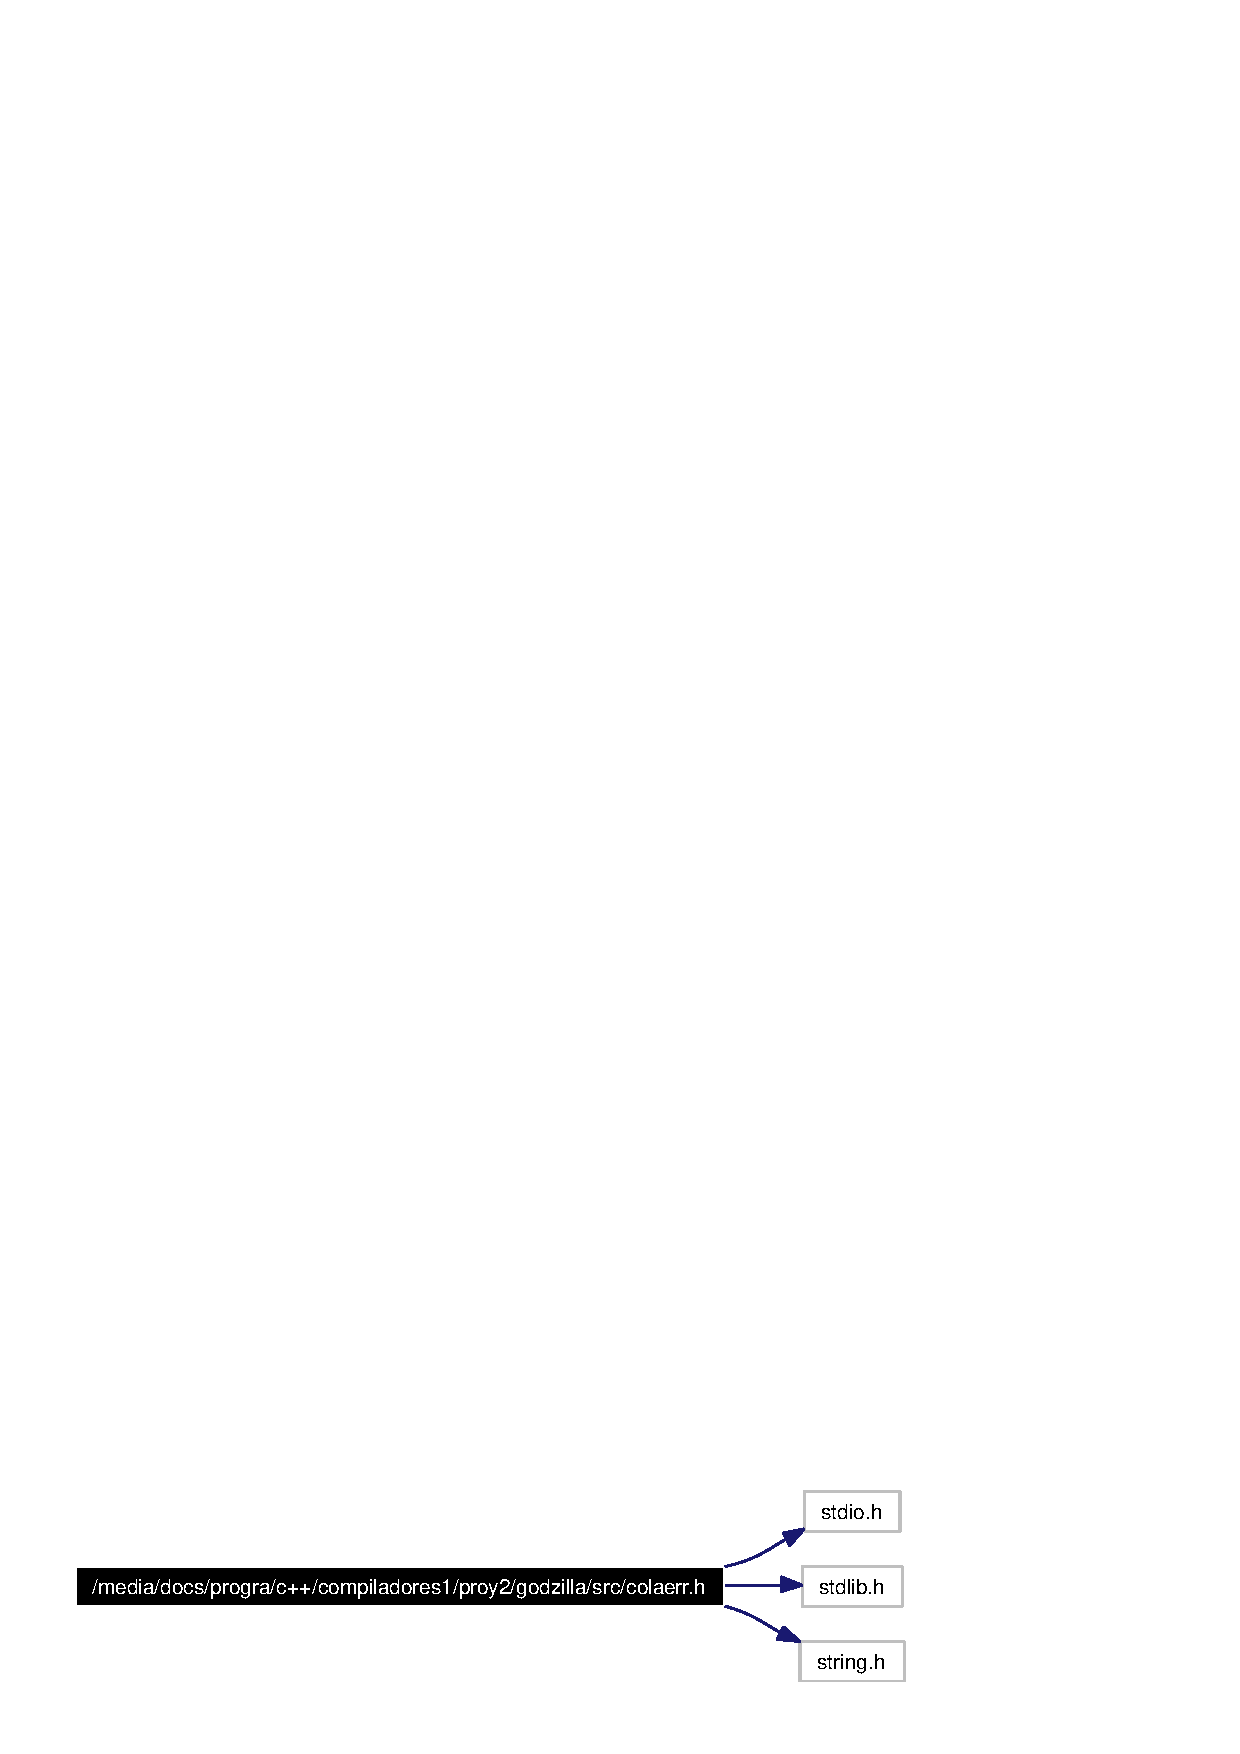
\includegraphics[width=217pt]{colaerr_8h__incl}
\end{center}
\end{figure}


Este gr\'{a}fico muestra que archivos directa o indirectamente incluyen a este archivo:\begin{figure}[H]
\begin{center}
\leavevmode
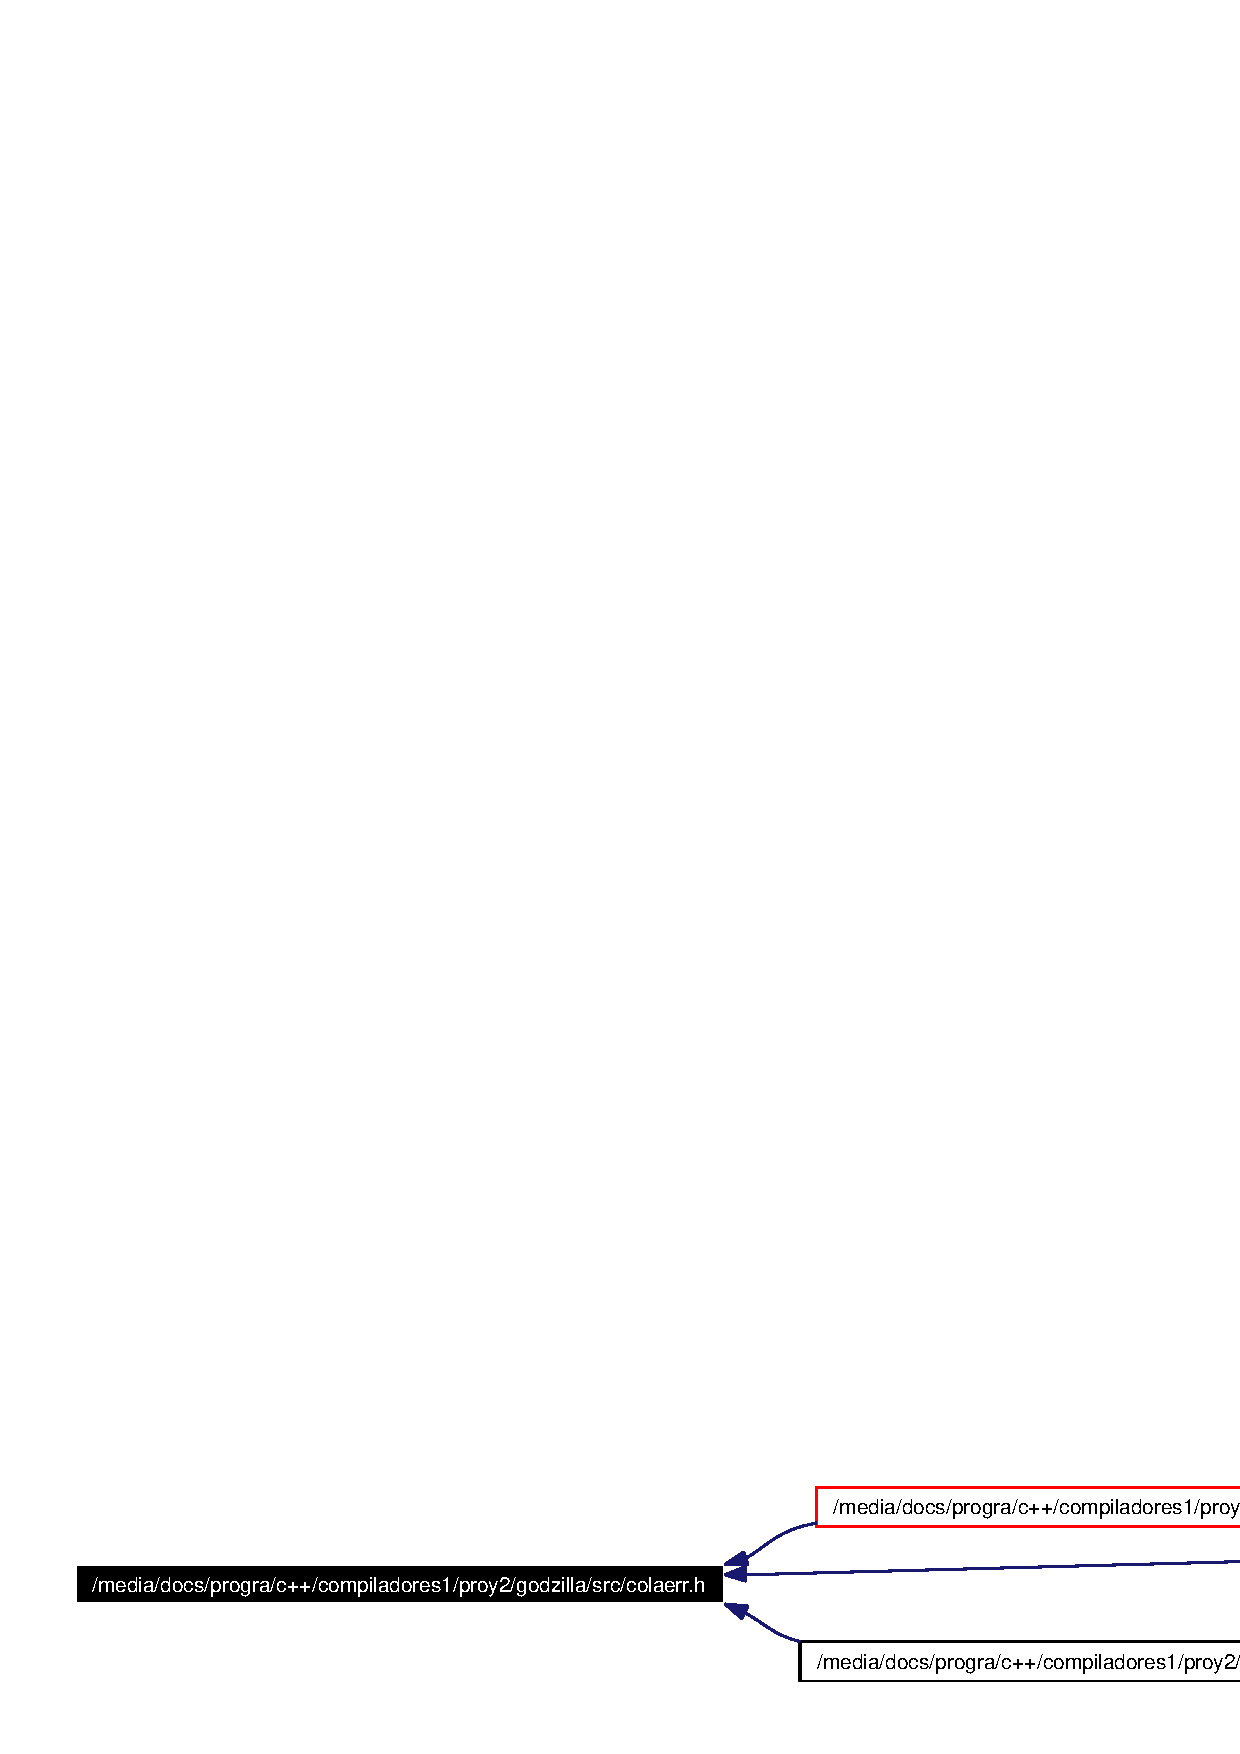
\includegraphics[width=420pt]{colaerr_8h__dep__incl}
\end{center}
\end{figure}
\subsection*{Clases}
\begin{CompactItemize}
\item 
struct {\bf tipo\-Error}
\begin{CompactList}\small\item\em Clase de almacenamiento de error. \item\end{CompactList}\item 
struct {\bf nodo\-Cola\-Err}
\begin{CompactList}\small\item\em Nodo de la cola de errores. \item\end{CompactList}\item 
struct {\bf cola\-Err}
\begin{CompactList}\small\item\em Cola de errores. \item\end{CompactList}\end{CompactItemize}
\subsection*{Tipos definidos}
\begin{CompactItemize}
\item 
typedef {\bf nodo\-Cola\-Err} {\bf nodo\-Cola\-Err}
\item 
typedef {\bf cola\-Err} {\bf cola\-Err}
\item 
typedef {\bf tipo\-Error} {\bf tipo\-Error}
\end{CompactItemize}
\subsection*{Funciones}
\begin{CompactItemize}
\item 
void {\bf encolar\-Error} ({\bf cola\-Err} $\ast$cerr, {\bf tipo\-Error} $\ast$err)
\begin{CompactList}\small\item\em Agrega un error a la cola de errores. \item\end{CompactList}\item 
{\bf tipo\-Error} $\ast$ {\bf sacar\-Error} ({\bf cola\-Err} $\ast$cerr)
\begin{CompactList}\small\item\em Agrega un error a la cola de errores. \item\end{CompactList}\item 
void {\bf error\-Lexico} (char $\ast$msg)
\begin{CompactList}\small\item\em Devuelve primer error en la cola de erroes. \item\end{CompactList}\item 
void {\bf error\-Sintactico} (char $\ast$msg)
\begin{CompactList}\small\item\em Agrega mensaje a la cola de errores lexicos. \item\end{CompactList}\item 
void {\bf error\-Semantico} (char $\ast$msg, int numlinea)
\begin{CompactList}\small\item\em Agrega mensaje a la cola de errores sintacticos. \item\end{CompactList}\item 
int {\bf escribir\-Error\-Log\-XML} (const char $\ast$filename)
\begin{CompactList}\small\item\em Agrega mensaje a la cola de errores semanticos. \item\end{CompactList}\end{CompactItemize}
\subsection*{Variables}
\begin{CompactItemize}
\item 
int {\bf line\_\-num}
\item 
int {\bf column}
\end{CompactItemize}


\subsection{Descripci\'{o}n detallada}
Definiciones de la cola almacenadora de errores . 



Definici\'{o}n en el archivo {\bf colaerr.h}.

\subsection{Documentaci\'{o}n de los tipos definidos}
\index{colaerr.h@{colaerr.h}!colaErr@{colaErr}}
\index{colaErr@{colaErr}!colaerr.h@{colaerr.h}}
\subsubsection{\setlength{\rightskip}{0pt plus 5cm}typedef struct {\bf cola\-Err} {\bf cola\-Err}}\label{colaerr_8h_a3}




Definici\'{o}n en la l\'{\i}nea 24 del archivo colaerr.h.\index{colaerr.h@{colaerr.h}!nodoColaErr@{nodoColaErr}}
\index{nodoColaErr@{nodoColaErr}!colaerr.h@{colaerr.h}}
\subsubsection{\setlength{\rightskip}{0pt plus 5cm}typedef struct {\bf nodo\-Cola\-Err} {\bf nodo\-Cola\-Err}}\label{colaerr_8h_a2}




Definici\'{o}n en la l\'{\i}nea 23 del archivo colaerr.h.\index{colaerr.h@{colaerr.h}!tipoError@{tipoError}}
\index{tipoError@{tipoError}!colaerr.h@{colaerr.h}}
\subsubsection{\setlength{\rightskip}{0pt plus 5cm}typedef struct {\bf tipo\-Error} {\bf tipo\-Error}}\label{colaerr_8h_a4}




Definici\'{o}n en la l\'{\i}nea 25 del archivo colaerr.h.

\subsection{Documentaci\'{o}n de las funciones}
\index{colaerr.h@{colaerr.h}!encolarError@{encolarError}}
\index{encolarError@{encolarError}!colaerr.h@{colaerr.h}}
\subsubsection{\setlength{\rightskip}{0pt plus 5cm}void encolar\-Error ({\bf cola\-Err} $\ast$ {\em cerr}, {\bf tipo\-Error} $\ast$ {\em err})}\label{colaerr_8h_a5}


Agrega un error a la cola de errores. 



Definici\'{o}n en la l\'{\i}nea 24 del archivo colaerr.c.

Hace referencia a nodo\-Cola\-Err::err, cola\-Err::primero, nodo\-Cola\-Err::siguiente, y cola\-Err::ultimo.

Referenciado por error\-Lexico(), error\-Semantico(), y error\-Sintactico().\index{colaerr.h@{colaerr.h}!errorLexico@{errorLexico}}
\index{errorLexico@{errorLexico}!colaerr.h@{colaerr.h}}
\subsubsection{\setlength{\rightskip}{0pt plus 5cm}void error\-Lexico (char $\ast$ {\em msg})}\label{colaerr_8h_a7}


Devuelve primer error en la cola de erroes. 



Definici\'{o}n en la l\'{\i}nea 53 del archivo colaerr.c.

Hace referencia a tipo\-Error::col, column, tipo\-Error::desc, encolar\-Error(), hubo\-Error\-Lexico, line\_\-num, y tipo\-Error::linea.\index{colaerr.h@{colaerr.h}!errorSemantico@{errorSemantico}}
\index{errorSemantico@{errorSemantico}!colaerr.h@{colaerr.h}}
\subsubsection{\setlength{\rightskip}{0pt plus 5cm}void error\-Semantico (char $\ast$ {\em msg}, int {\em numlinea})}\label{colaerr_8h_a9}


Agrega mensaje a la cola de errores sintacticos. 



Definici\'{o}n en la l\'{\i}nea 74 del archivo colaerr.c.

Hace referencia a tipo\-Error::col, tipo\-Error::desc, encolar\-Error(), hubo\-Error\-Semantico, y tipo\-Error::linea.

Referenciado por error().\index{colaerr.h@{colaerr.h}!errorSintactico@{errorSintactico}}
\index{errorSintactico@{errorSintactico}!colaerr.h@{colaerr.h}}
\subsubsection{\setlength{\rightskip}{0pt plus 5cm}void error\-Sintactico (char $\ast$ {\em msg})}\label{colaerr_8h_a8}


Agrega mensaje a la cola de errores lexicos. 



Definici\'{o}n en la l\'{\i}nea 63 del archivo colaerr.c.

Hace referencia a tipo\-Error::col, column, tipo\-Error::desc, encolar\-Error(), hubo\-Error\-Sintactico, line\_\-num, y tipo\-Error::linea.\index{colaerr.h@{colaerr.h}!escribirErrorLogXML@{escribirErrorLogXML}}
\index{escribirErrorLogXML@{escribirErrorLogXML}!colaerr.h@{colaerr.h}}
\subsubsection{\setlength{\rightskip}{0pt plus 5cm}int escribir\-Error\-Log\-XML (const char $\ast$ {\em filename})}\label{colaerr_8h_a10}


Agrega mensaje a la cola de errores semanticos. 



Definici\'{o}n en la l\'{\i}nea 84 del archivo colaerr.c.

Hace referencia a tipo\-Error::col, tipo\-Error::desc, errfile, tipo\-Error::linea, cola\-Err::primero, y sacar\-Error().\index{colaerr.h@{colaerr.h}!sacarError@{sacarError}}
\index{sacarError@{sacarError}!colaerr.h@{colaerr.h}}
\subsubsection{\setlength{\rightskip}{0pt plus 5cm}{\bf tipo\-Error}$\ast$ sacar\-Error ({\bf cola\-Err} $\ast$ {\em cerr})}\label{colaerr_8h_a6}


Agrega un error a la cola de errores. 



Definici\'{o}n en la l\'{\i}nea 36 del archivo colaerr.c.

Hace referencia a nodo\-Cola\-Err::err, cola\-Err::primero, nodo\-Cola\-Err::siguiente, y cola\-Err::ultimo.

Referenciado por escribir\-Error\-Log\-XML().

\subsection{Documentaci\'{o}n de las variables}
\index{colaerr.h@{colaerr.h}!column@{column}}
\index{column@{column}!colaerr.h@{colaerr.h}}
\subsubsection{\setlength{\rightskip}{0pt plus 5cm}int {\bf column}}\label{colaerr_8h_a1}




Referenciado por error\-Lexico(), y error\-Sintactico().\index{colaerr.h@{colaerr.h}!line_num@{line\_\-num}}
\index{line_num@{line\_\-num}!colaerr.h@{colaerr.h}}
\subsubsection{\setlength{\rightskip}{0pt plus 5cm}int {\bf line\_\-num}}\label{colaerr_8h_a0}




Referenciado por error\-Lexico(), y error\-Sintactico().